%! TEX root = /home/hsartoris/sproj/writeup/main.tex
\graphicspath{ {resources/} }
\chapter{Model}
\label{model}
The model trained and tested here represents ... stuff

\section{Data}
\label{sec:data}
Insofar as we treat ANNs as providing arbitrary function approximation, training
a network requires input data representing the known data about the system we
wish to model, as well as output data we wish the network to produce from the
inputs. More generally, input data usually entails information that is easy to 
acquire about the process being modeled, while output data, or labels, 
correspond to a dataset that is difficult to acquire generally. Of course, this 
means that the first step in training a neural network is to assemble a 
sufficiently large set of inputs and outputs in order to fully, or at least 
approximately, characterize the problem at hand.

In our case, we wish to map from (relatively) easily available data about 
biological networks, individual neuron spike times, to network structure. While 
such data exist, generating our own allows us to better analyze the results of 
the algorithm.


\subsection{Generation}
In order to demonstrate the validity of our algorithm for graph convolution, we 
opt for a simplified form of the kind of data that would be used in a real-world 
setting.  To this end, we create adjacency matrices representing simple, 
small-\textit{n} toy networks.

\begin{table}[h]
	\centering
	
\begin{tikzpicture}[baseline=(current bounding box.center),->,>=stealth', 
	node distance=5em, semithick]
	\tikzstyle{every state}=[fill=none, draw=black, text=black]

	\node[state] (0) {0};
	\node[state] (1) [right of=0] {1};
	\node[state] (2) [below right of=0] {2};

	\path 	(0) edge node {} (1)
			(0) edge node {} (2)
			(1) edge node {} (2);
\end{tikzpicture}

	\hspace{2em}
	\begin{tabular}{l|lll}
		  & 0 & 1 & 2\\
		\hline
		0 & 0 & 0 & 0\\
		1 & 1 & 0 & 0\\
		2 & 1 & 1 & 0
	\end{tabular}
	\captionof{figure}{Example of 3-neuron network and adjacency matrix.}
	\label{fig:toyex}
\end{table}\noindent
Binary values are used throughout these toy networks: either a connection exists 
or it doesn't; either a `neuron' is spiking or it isn't. To produce spiking 
data, we create an \textit{n}-vector $\mathbb{S}$ representing the current state 
of the toy network, with random neurons already spiking based on a chosen spike 
rate. From here, the process is as in \ref{subsec:adjacency}, where $\mathbb{M}$ 
is the adjacency matrix:

\[
	\underset{n \times n}{\mathbb{M}} \times \underset{n \times 1}{\mathbb{S}^t} 
	= \underset{n \times 1}{\mathbb{S}^{t+1}}
\]
Additonally, $\mathbb{S}^{t+1}$ may have one or more neurons spike randomly, as 
determined by the spike rate of the simulation.\footnote{SEE APPENDIX} All 
values are clipped to the range $[0,1]$, to avoid double spiking.

At each step, $\mathbb{S}$ is appended to an output matrix, which is saved after 
simulation is complete. For $t$ simulation steps, the completed output has shape 
$(n \times t)$.

\subsubsection{Example Data Generation}
Consider the network defined in figure \ref{fig:toyex}. Supposing that we 
randomly spike neuron 0 at the first step, our initial state appears as such, 
where $\mathbb{O}$ is the output matrix and $\mathbb{R}$ is an \textit{n}-vector 
wherein each element has been randomly assigned 0 or 1, based on the spike rate 
of the simulation:
\[
	\mathbb{M} = \begin{bmatrix}
		0 & 0 & 0 \\
		1 & 0 & 0 \\
		1 & 1 & 0
	\end{bmatrix} \qquad
	\mathbb{S}^0 = \begin{bmatrix} 1 \\ 0 \\ 0 \end{bmatrix} \qquad
	\mathbb{O} = \begin{bmatrix} 1 \\ 0 \\ 0 \end{bmatrix}
\]
We now compute $\mathbb{S}^1$ as above:
\[
	\mathbb{S}^1 = (\mathbb{M} \times \mathbb{S}^0) + \mathbb{R} = 
		\left(\begin{bmatrix}
		0 & 0 & 0 \\
		1 & 0 & 0 \\
		1 & 1 & 0
	\end{bmatrix} \times \begin{bmatrix} 1 \\ 0 \\ 0 \end{bmatrix}\right)
	+ \begin{bmatrix} 0 \\ 1 \\ 0 \end{bmatrix}
	= \begin{bmatrix} 0 \\ 2 \\ 1 \end{bmatrix}
\]
In this case, neuron 1 was spiked randomly, but was also spiked by virtue of its 
connection from 0. Since in this simple model we only consider neurons to be 
either spiking or not, binary values, we clip the values in $\mathbb{S}^1$ to a 
maximum of 1, in order to prevent cases such as this one from causing spikes of 
greater magnitude to propagate through the network. This also prevents neurons 
from double spiking due to multiple inputs being active in the same timestep. 
Thus we have our final value for $\mathbb{S}^1$, and append it to $\mathbb{O}$.
\[
	\mathbb{S}^1 = \begin{bmatrix} 0 \\ 1 \\ 1 \end{bmatrix} \qquad
	\mathbb{O} = \begin{bmatrix}
		1 & 0\\
		0 & 1\\
		0 & 1 \end{bmatrix}
\]
If we were to repeat this process several more times, we might end up with an 
output matrix such as in figure \ref{fig:exoutput}.
\begin{figure}[H]
\[
	\mathbb{O} = \begin{bmatrix}
		1 & 0 & 1 & 0 & 0\\
		0 & 1 & 0 & 1 & 0\\
		0 & 1 & 1 & 1 & 1
	\end{bmatrix}
\]
\caption{Example output matrix for a 3-neuron network simulated for five steps.}
\label{fig:exoutput}
\end{figure}\noindent
We can clearly see the effects of neuron 2 having inputs from both other 
neurons. Practically, the number of iterations was usually set to 50.

\subsection{Generalizability}
\label{subsec:hotswap}
In most ANN implementations, feeding various data with the same label attached 
to it results in the network learning to ignore the input data and always return 
the desired label, rendering it useless. However, due to the unique structure of 
our model, this sort of overfitting is impossible (SEE SOME ARCHITECTURE 
SECTION).  Therefore, we must merely construct a suitably representative 
generator network, meaning that it contains all of the inter-neuron 
relationships we expect to see in the data we ultimately feed in to test.

\subsection{Restructuring}
The model accepts data in the form of a spike-time raster plot of dimensions $(n 
\times t)$, where \textit{n} is the number of neurons and \textit{t} is the 
number of timesteps being considered. The axes are reversed in comparison to the 
data created by the generator, and thus in the process of loading in the spike 
trains we transpose the matrices to the expected dimensionality. Additionally, 
it is not always necessary to use the full number of steps generated, depending 
on the size of the generator network in question, as well as its spike rate. In 
such a scenario, we truncate the time dimension appropriately.

For a network accepting \textit{t} timesteps of data from \textit{n} neurons, 
the data fed into the network takes the following form:
\[ \begin{bmatrix}
		x_{11} & x_{12} & \dots & x_{1n}\\
		x_{21} & x_{22} & \dots & x_{2n}\\
		\vdots & \vdots & \ddots & \vdots\\
		x_{t1} & x_{t2} & \dots & x_{tn}
	\end{bmatrix} \]
Applying this process to the data in figure \ref{fig:exoutput}, including 
truncating the time dimension to four, results in the following:
\begin{figure}[H]
	\centering
	\begin{subfigure}{.48\textwidth}
		\[
			\begin{bmatrix}
				1 & 0 & 0\\
				0 & 1 & 1\\
				1 & 0 & 1\\
				0 & 1 & 1
			\end{bmatrix}
		\]
		\caption{Transposed output matrix}
	\end{subfigure}
	\begin{subfigure}{.48\textwidth}
		\centering
		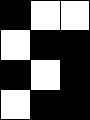
\includegraphics[width=.35\textwidth]{3outex.png}
		\caption{Graphical representation}
		\label{subfig:3outexgraph}
	\end{subfigure}
	\caption{Transposed and truncated matrix and associated visualization.}
\end{figure}\noindent
The representation of the matrix in \ref{subfig:3outexgraph} is an example of 
the method we will use to depict matrices containing real values.

\section{Architecture}
We will first describe the architecture in terms that, while accurate on the 
macro level, do not fully reflect the actual transformations occuring in the 
implemented model. We will then proceed to a mathematically representative 
version, leaving explanation of the batched version of the model to APPENDIX 
SECTION.

\subsection{Structure \& Computation Details}
\subsubsection{Dimensionality-defining Variables}
Only two values characterize the matrices and transitions involved in the model.  
They are as follows:
\begin{description}
	\item \textit{b}: The number of steps of input data the model considers in a 
		given piece of data.
	\item \textit{d}: The length of the vectors characterizing each potential 
		connection \textit{ij}. This restricts the maximum information about 
		each potential neuron pair that the model can maintain across layer 
		transitions.
\end{description}
We determined effective values for these parameters through experimentation.

Additionally, we use the number of nodes in the generator graph, \textit{n}, to 
calculate summations and averages, but the structure of our calculations is such 
that no aspects of the model are defined in terms of \textit{n}.

\subsubsection{Activation Functions}
At the end of each transition, an elementwise activation function\footnote{SEE 
THE PART OF THE BG WHERE I TALK ABOUT NN PRINCIPLES} is applied following 
completion of all computations.  For all but the final layer, that function is 
ReLU\footnote{NEEDS CITATION}, which is defined as follows:
\begin{equation}
	relu(x) = \begin{cases}
		0 & x < 0\\
		x & x \geq 0
	\end{cases}
\end{equation}

\subsection{First Transition}
To generate the first layer of the network, we inspect every pair of neurons in 
the input data. Since no pair of neurons is distinguishable from another, the 
comparison applied is the same in all cases: we apply the same convolutional 
filter to all pairs. We achieve this by concatenating the spike train of each 
neuron \textit{i} individually with every other neuron \textit{j}, then 
multiplying by a matrix $\mathbb{W}$ of dimensionality $(d \times 
2b)$.\footnote{Recall that the time dimension fed into the network is 
characterized by \textit{b}.}

$\mathbb{W}$ is trained on, and thus the comparison of each pair of spike trains 
is left up to the network. The transition appears as follows, where $\underset{b 
\times 1}{\mathbb{I}_x}$ is the input column at \textit{x}:
\[
	\mathlarger\forall i,j \mid 0 \leq i,j < n: \underset{d \times 
	1}{d_{ij}^\prime} = \underset{d \times 2b}{\mathbb{W}} \times 
	\left(\frac{\mathbb{I}_i}{\mathbb{I}_j}\right)
\]
This leaves us with $n^2$ \textit{d}-vectors, each characterizing one potential 
edge \textit{ij}.

\subsection{Convolutional Layer}
In this layer, we incorporate information from all nodes potentially adjacent to 
each edge \textit{ij}. From our previous layer, we have a matrix of shape $(d 
\times n^2)$ that we will refer to as $\mathbb{D}^{\prime}$, but it will be 
useful to keep in mind an alternate representation of that matrix, one in three 
dimensions, which we shall refer to as $\mathbb{D}_N^{\prime}$.

\begin{figure}[H]
\begin{tikzpicture}
    \pgfmathsetmacro{\n}{20}
    \pgfmathsetmacro{\t}{40}
    \pgfmathsetmacro{\d}{12}
    \pgfmathsetmacro{\scale}{.07}
	\pic at (2,-1) {annotated cuboid={width=\n*4, height=3, depth=\d, xlabel=n, 
	ylabel=1, zlabel=d, scale=\scale}};
    \node at (3.7,-1) {\scalebox{2}{$\Leftrightarrow$}};
	\pic at (6.8,-.27) {annotated cuboid={width=\n, height=\n, depth=\d, 
xlabel=n, ylabel=n, zlabel=d, scale=\scale}};
	\node at (-.8, -3)  {\scalebox{1.5}{$\mathbb{D}^{\prime}$}};
	\node at (6.3, -3) {\scalebox{1.5}{$\mathbb{D}_N^{\prime}$}};
\end{tikzpicture}
\caption{Relationship between $\mathbb{D}^{\prime}$ and 
$\mathbb{D}^{\prime}_N$.}
\end{figure}\noindent
Consider some $d_{ij}^{\prime}$ in $\mathbb{D}^{\prime}_N$. Then we can say the 
following:
\begin{enumerate}
	\item $d_{ij}^{\prime}$ represents the connection from \textit{j} to 
		\textit{i} as it may or may not exist in this network, in the form of 
		\textit{d} values of indeterminate meaning
	\item $\mathlarger\forall k \mid 0 \leq k < n$, $d_{jk}^{\prime}$ represents 
		a potential input to \textit{j}
	\item $\mathlarger\forall k \mid 0 \leq k < n$, $d_{ki}^{\prime}$ represents 
		a potential output from \textit{i}
\end{enumerate}
In our determination of the presence or absence of a connection from \textit{j} 
to \textit{i}, we wish to incorporate information from these potentially 
connected nodes; i.e., these inputs and outputs represent potential neighbors in 
a graph locality sense. To achieve this, we perform the following 
computations\footnote{Actually, it's much more elegant.} for each $\underset{d 
\times 1}{d_{ij}}$:
\begin{gather}
	\begin{align}
		\label{eq:ID}
		\underset{d \times 1}{\mathbb{I}} &= \frac{1}{n} \sum_{k=0}^{n-1} 
		d_{jk}^{\prime} & \underset{d \times 1}{\mathbb{O}} &= \frac{1}{n} 
		\sum_{k=0}^{n-1} d_{ki}^{\prime}\\
		\label{eq:IDOD}
	\underset{d \times 1}{\mathbb{I_D}} &= \underset{d \times 
	d}{\mathbb{W}_{in}^\prime} \times \left(\mathbb{I} \odot 
d_{ij}^{\prime}\right) & \underset{d \times 1}{\mathbb{O_D}} &= \underset{d 
\times d}{\mathbb{W}_{out}^\prime} \times \left(\mathbb{O} \odot 
d_{ij}^{\prime}\right)
	\end{align}
	\shortintertext{\centering Here we arrive at the output,
	$d_{ij}^{\prime\prime}$:}
	d_{ij}^{\prime\prime} = \underset{d \times 2d}{\mathbb{W}_{tot}^\prime} 
	\times \left(\frac{\mathbb{I_D}}{\mathbb{O_D}}\right) \label{eq:dijO}
\end{gather}
Conceptually, in \eqref{eq:ID} we first average all potential inputs to and 
outputs from potential edge \textit{ij}. Then, we compute an entrywise product 
($\odot$) of these vectors with the vector describing the edge in question, 
$d_{ij}^{\prime}$. While we have integrated locality data into the results thus 
far, the network has not been allowed any processing over the resultant data, 
which we rectify by multiplying the input and output vectors with separate 
dimensionality-preserving $(d \times d)$ matrices. We thus arrive at 
\eqref{eq:IDOD}, with vectors $\mathbb{I_D}$ and $\mathbb{O_D}$ representing 
edge \textit{ij} with inputs and outputs, respectively, taken into 
consideration. In \eqref{eq:dijO}, we arrive at $d_{ij}^{\prime\prime}$ as it 
will be seen by the next layer of the network by multiplying a third weight 
matrix by the vertical concatenation of $\mathbb{I_D}$ and $\mathbb{O_D}$.  This 
matrix $\mathbb{W}_{tot}^\prime$, allows the network to optimize for whichever 
elements in $\mathbb{I_D}$ and $\mathbb{O_D}$ are most important in the 
prediction of \textit{ij}. The three matrices involved, 
$\mathbb{W}_{in}^\prime$, $\mathbb{W}_{out}^\prime$, and 
$\mathbb{W}_{tot}^\primt$, are trained on by the optimizer\footnote{SEE 
OPTIMIZER SECION IN TRAINING}, allowing the model to learn optimal processing 
and combinations to facilitate predictions.

Our concatenation approacb in \eqref{eq:dijO} stands in contrast to the strategy 
taken in \eqref{eq:IDOD}, where integration of the input and output data is 
forced via entrywise product computation. While we considered the same 
concatenation process for use in \eqref{eq:IDOD}, the apparent difficulty of 
integrating the calculated locality data into the prediction of \textit{ij} led 
the model to rapidly adapt its weight matrices to ignore the locality portion of 
the data.  For more discussion on this difficulty, see TRAINING SECTION.

Note again that none of the computations involved in this layer are dependent on 
\textit{n}; as the summations are averaged, the values contained in their 
resultant vectors will be of similar magnitude for any number of neurons under 
consideration. After executing this algorithm for each $d_{ij}^{\prime}$, we are 
left with another $(d \times n^2)$ output matrix, $\mathbb{D}^{\prime\prime}$.

\subsection{Final Transition}
The shift from $(d \times n^2)$ is comparatively simple, being only a 
dimensionality reduction:
\begin{equation}
	\mathlarger\forall d_{ij}^{\prime\prime} \in \mathbb{D}^{\prime\prime}:
	\underset{1 \times 1}{d_{ij}^f} = \underset{1 \times d}{\mathbb{W}^f} \times 
	\underset{d \times 1}{d_{ij}^{\prime\prime}}
\end{equation}
This leaves us with a $(1 \times n^2)$ matrix, which, following application of a 
hyperbolic tangent activation function and transposition to $(n \times n)$, we 
treat as the adjacency matrix of the generator associated with the input data.
